\section{Results sample}
\label{sec:results_sample}

In this section we present the main results the sample part.


\paragraph{Sample spectra}
%
In this work we will study the local electronic properties
via a low-loss region analysis of EELS taken on
WS$_2$ nanostructures.
%
WS$_2$ is a highly promising material exhibiting a wide range of 
possible applications for electronic and optical devices.
%
When WS$_2$ is thinned down to a single monolayer, its 
indirect band gap switches to a direct band gap of approximately 2 eV~\ref{table:bgvalues}.


\begin{table}[h]
  \caption{Literature values for the bandgap of monolayer and bulk WS$_2$}
  \begin{indented}
\item[]\begin{tabular}{@{}lll}
\br
Entry {[}reference{]}                       & Type & Band gap energy (eV) \\
\mr
\multirow{2}{*}{1 \cite{Gusakova:2007}} & ML   & 2.03                 \\
                                            & Bulk & 1.32                 \\
2 \cite{Kam:1982}                  & ML   & 1.79                 \\
                                            & Bulk & 1.35                 \\
3 \cite{Jo:2014}                 & ML   & 2.14                 \\
                                            & Bulk & 1.40                 \\ 
\br                                         
\end{tabular}
\end{indented}
\label{table:bgvalues}
\end{table}


\begin{figure}[h]
\begin{centering}
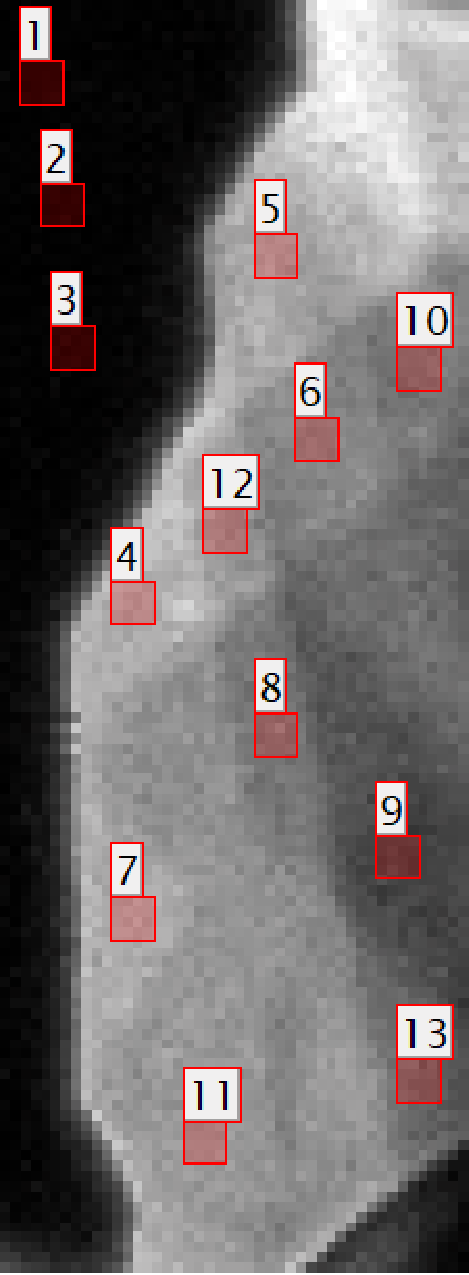
\includegraphics[width=0.2\linewidth]{plots/spectrumpositions.pdf} 
\caption{A specimen image of the WS$_2$ nanostructures. 
Marked are the positions at which energy loss data were obtained.}
\label{fig:ws2positions}
\end{centering}
\end{figure}
%
A collection of electron loss spectra acquired at different positions 
at the specimen is used to construct the neural network training inputs. 
%
These sets of data were obtained directly from~\cite{SabryaWS2}.
%
A specimen image of the positions can be observed in figure~\ref{fig:ws2positions}.  
This nanostructure exhibits flat layers with different thicknesses, which 
can be distinguished from the picture as color differences.
%
Energy loss spectra obtained at positions 1-3 are vacuum recordings, 
positions 4-13 represent in-sample data.
%
One layer (S-W-S) WS$_2$ has a thickness of around 0.9 nm. 
The thickness of the specimen at location 5 is 2.11 nm ($\sim$2 layers).
%
\begin{figure}[ht]
\begin{centering}
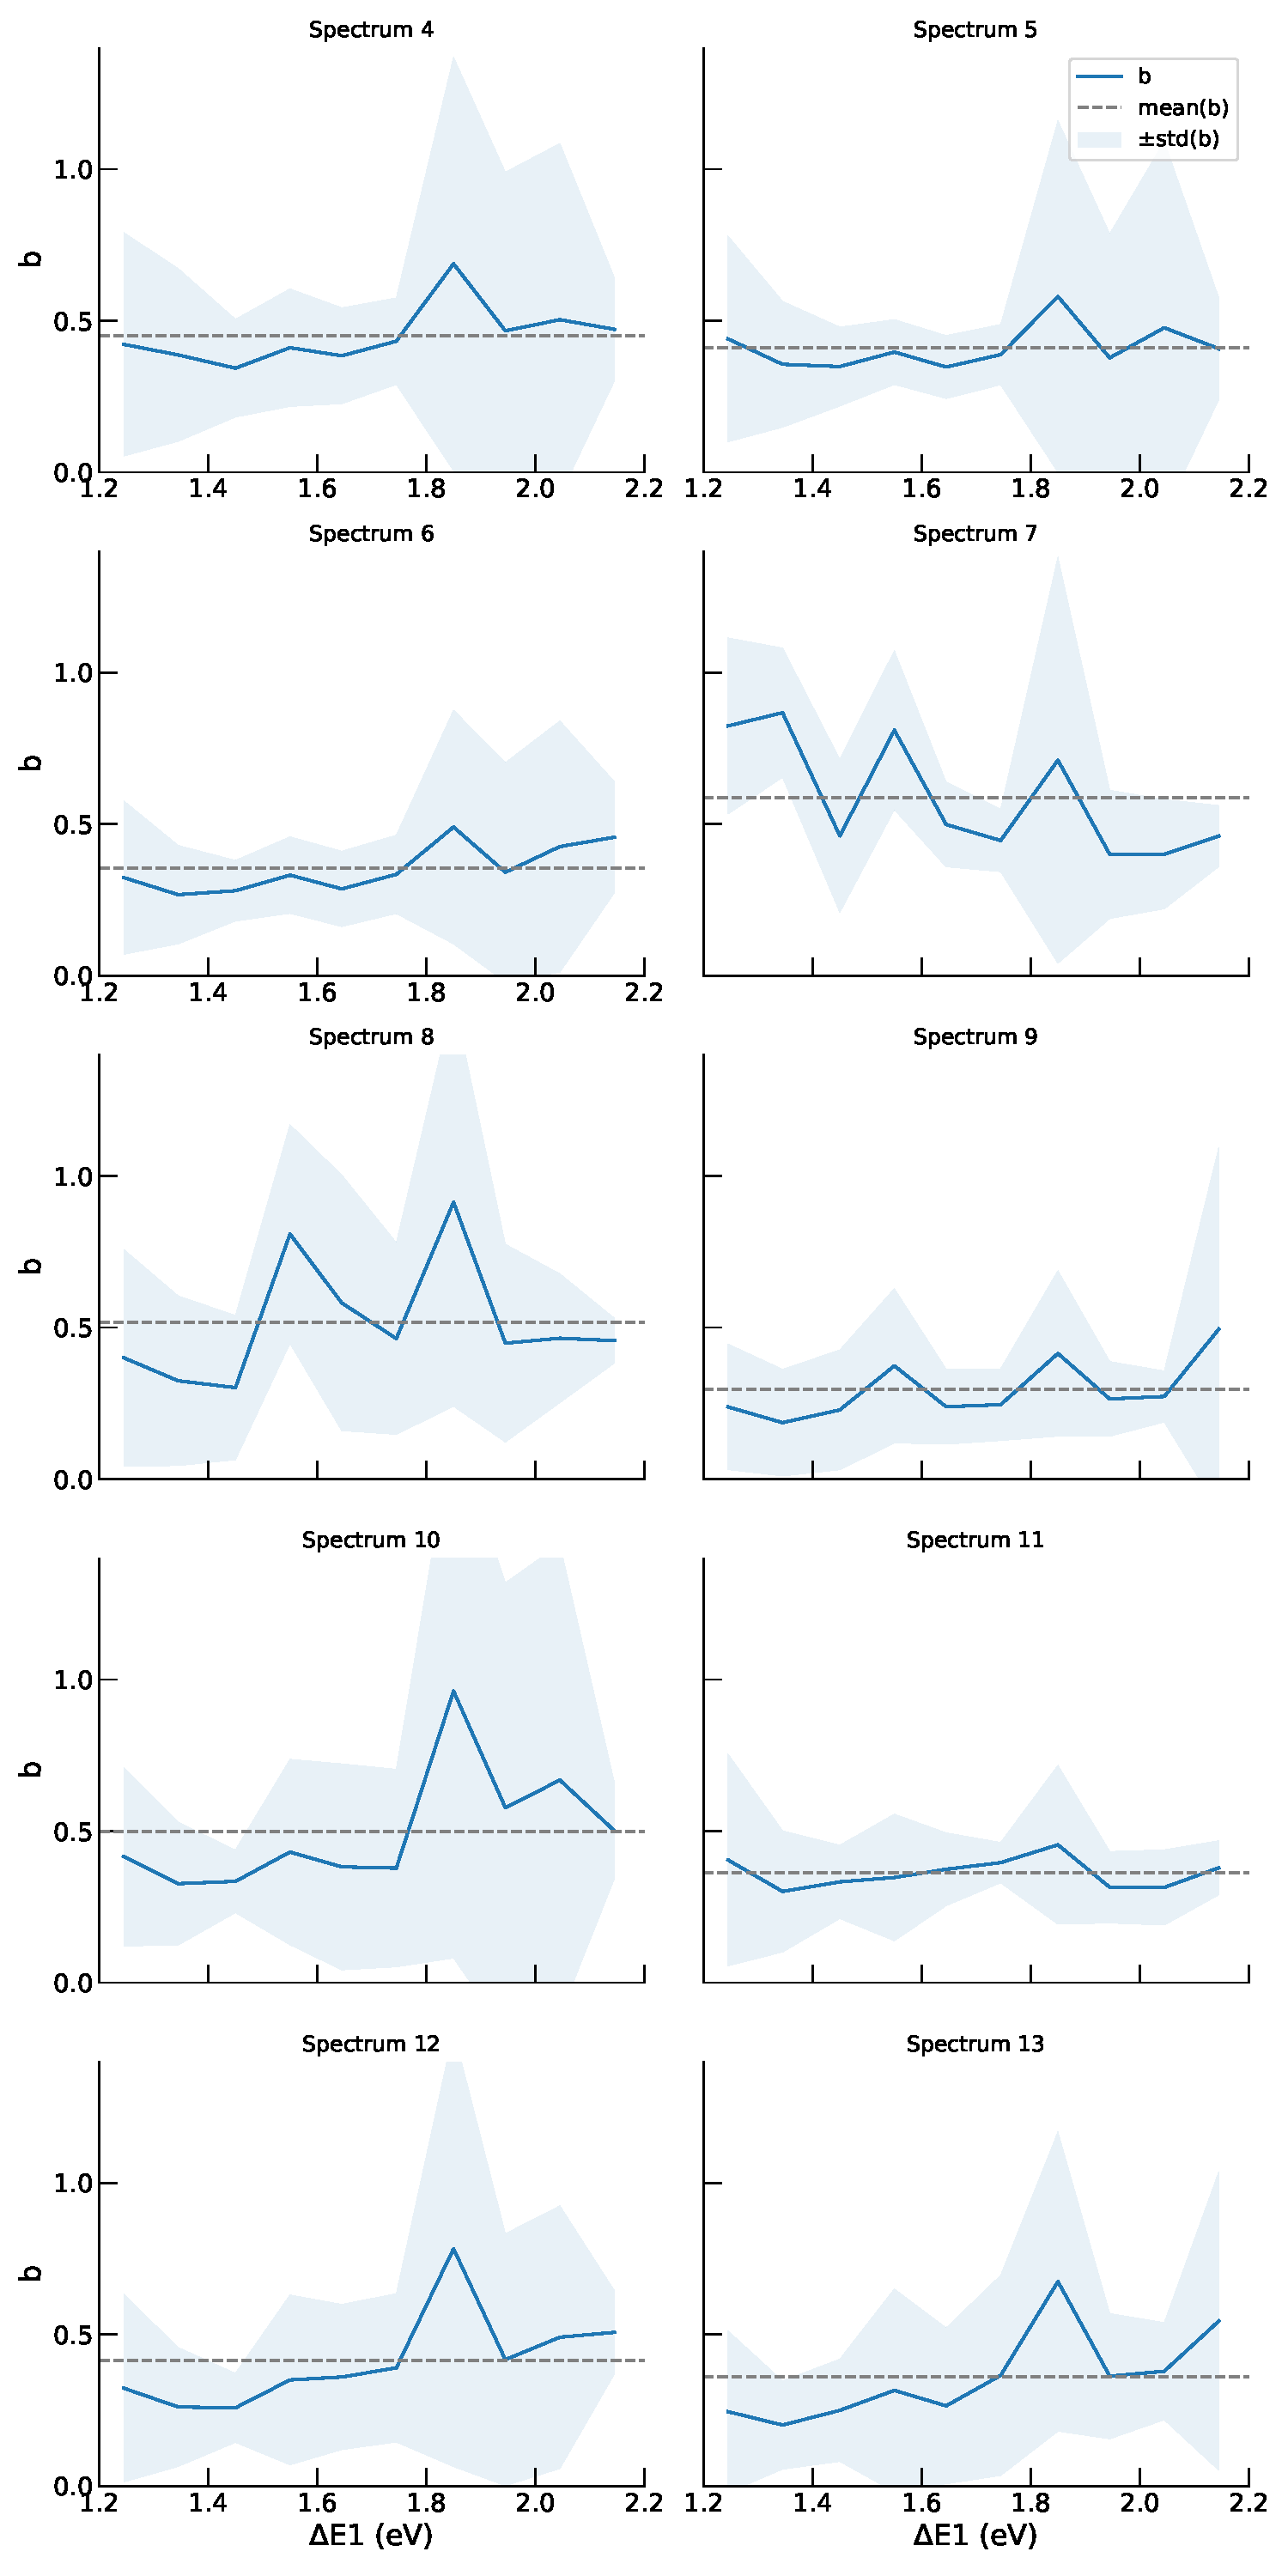
\includegraphics[width=0.6\linewidth]{plots/bvalues.pdf} 
\caption{Values for b at different positions}
\label{fig:bvalues}
\end{centering}
\end{figure}

\begin{figure}[ht]
\begin{centering}
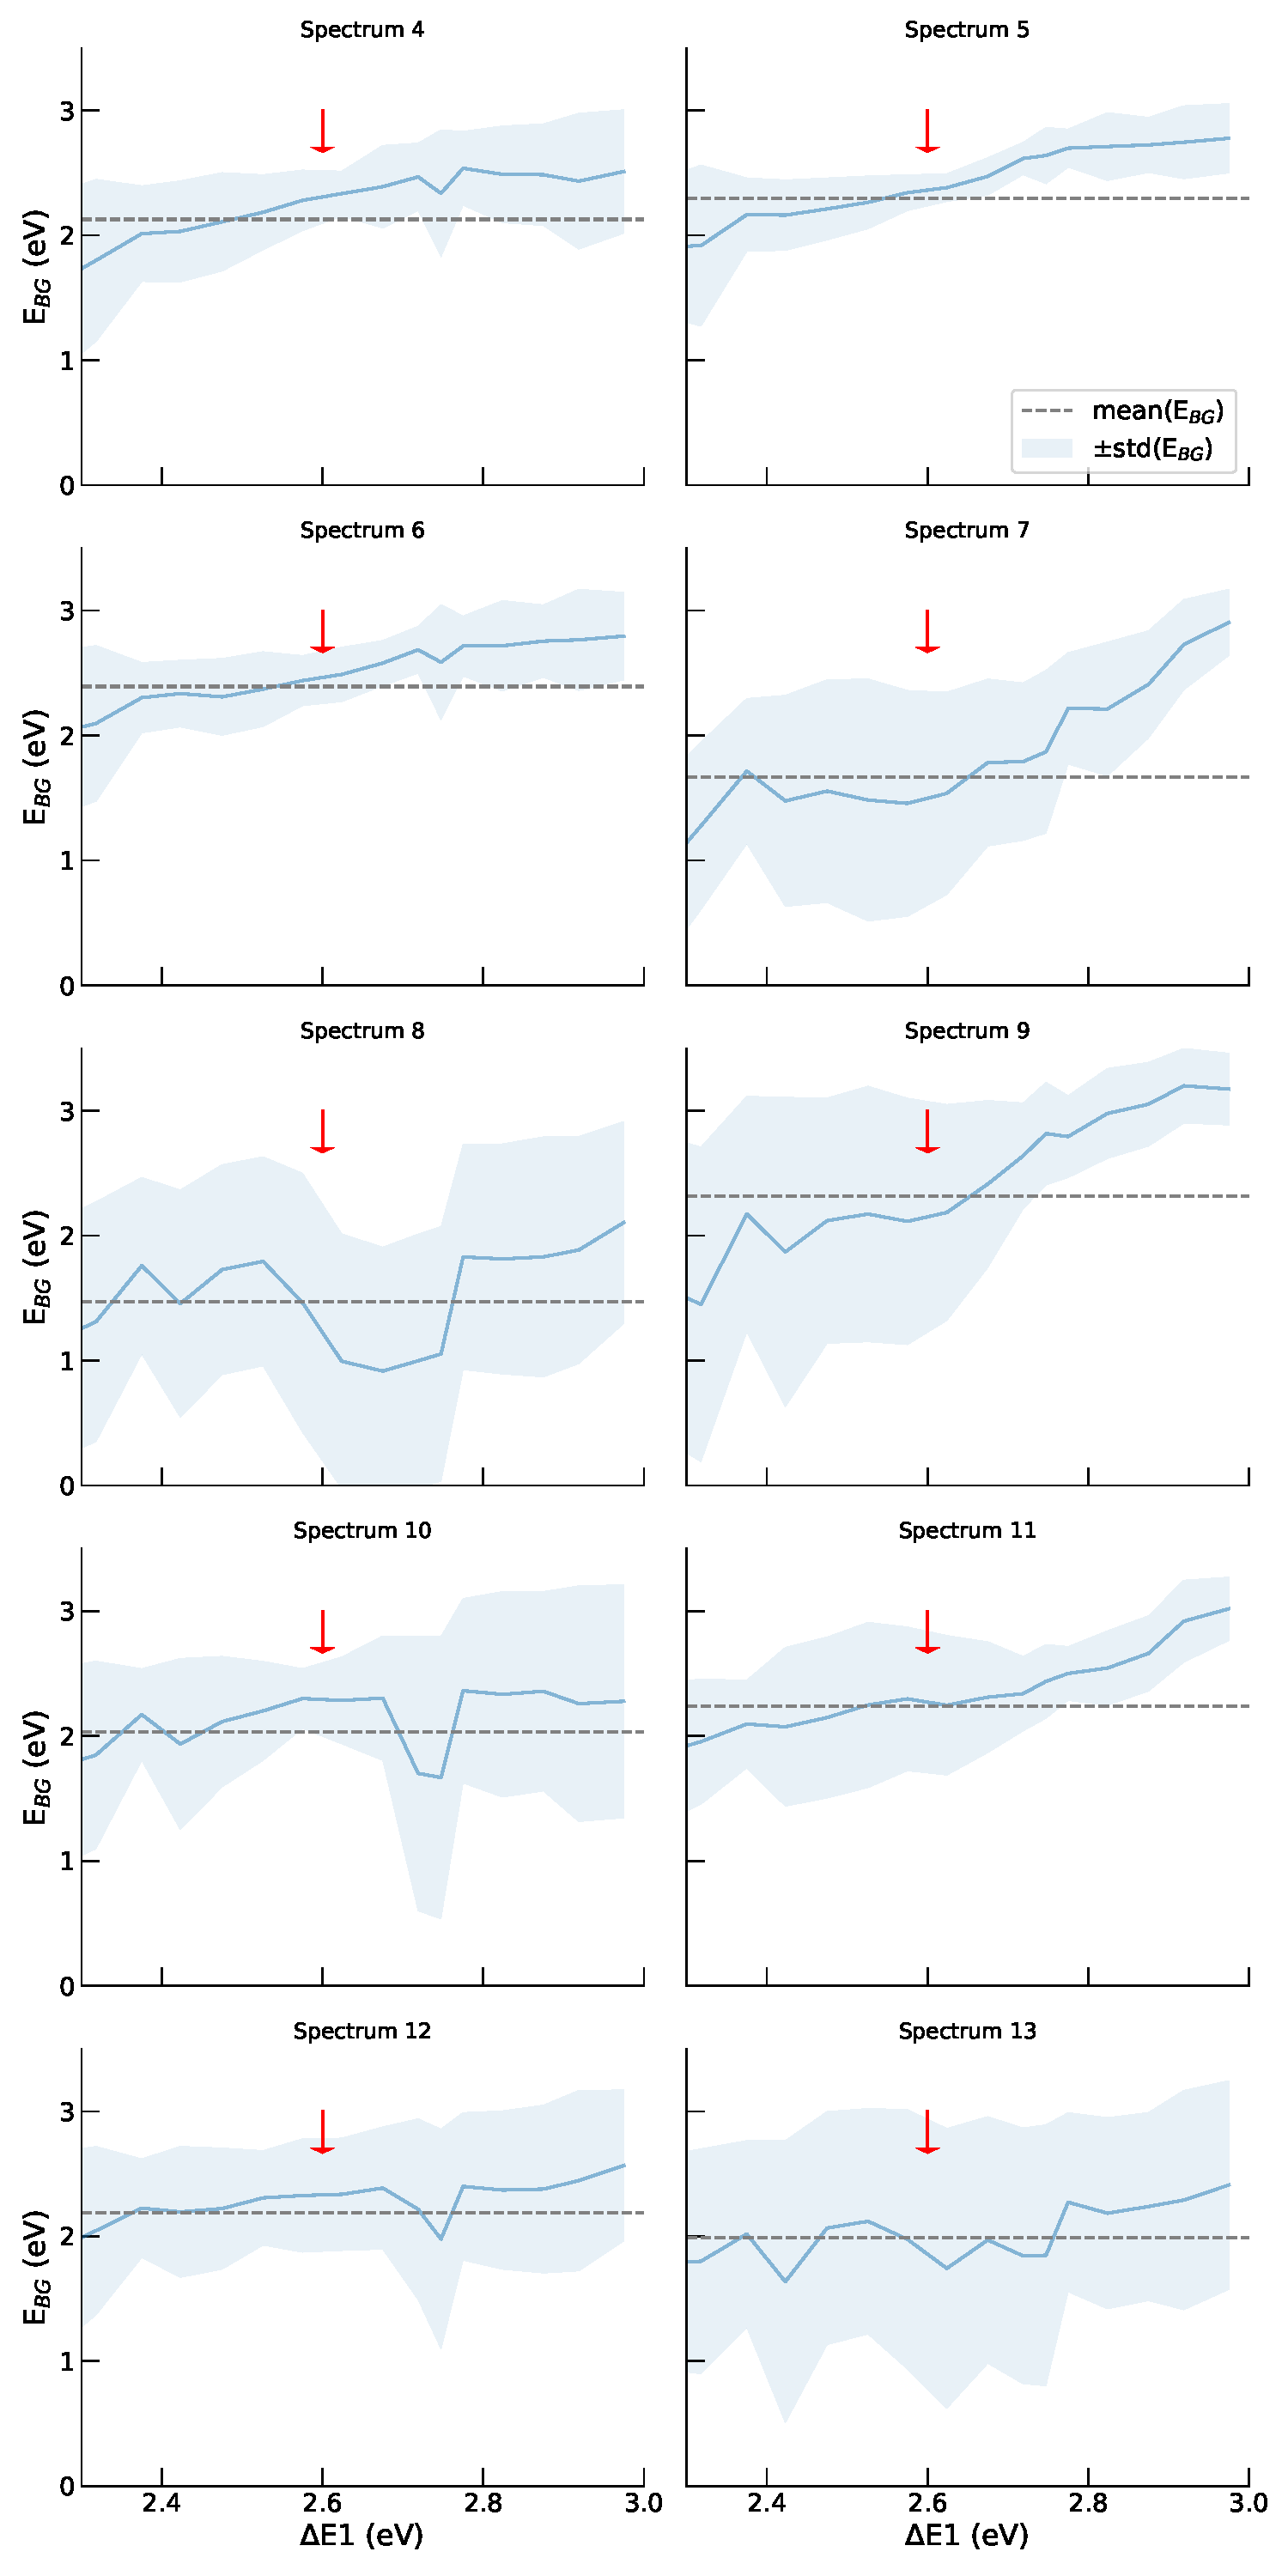
\includegraphics[width=0.6\linewidth]{plots/bgvalues.pdf} 
\caption{Values for E$_{BG}$ at different positions}
\label{fig:bvalues}
\end{centering}
\end{figure}




\subsection{Band-gap determination}


For each replica, the predicted ZLP is subtracted from the individual 
experimental spectra to obtain one set of subtractions. 
Repeating this procedure yields a collection of $N_{rep}$ subtractions 
for each original spectrum, over which statistical properties such as 
median and variance can be calculated.\newline
%
From these subtractions, which contain the 'pure' sample data, 
it is possible estimate the band gap. To a first approximation,
this can be done as the inflection point of the rising intensity.
%
The value can also be roughly estimated from the onset of the absorption 
or from a linear fit to the maximum positive slope in the 
EELS spectrum~\cite{Schamm:2003}. 
%
However, a more accurate and reliable determination is based on the work of 
Rafferty and Brown~\cite{Rafferty:2000}. The onset of the subtracted spectrum 
for a a material with a direct bandgap is expected to follow a function of the type
\begin{equation}\label{eq:I1}
    I(E) = I_0 + c\cdot(dE-E_{BG})^{(b)}
\end{equation}
where I$_0$ and c are constants, b equals 0.5, $\Delta$E is the energy loss and E$_{BG}$ 
is the bandgap energy.For an indirect bandgap, the power of $(1/2)$ changes to $(3/2)$. 
%
Therefore, the bandgap nature (direct or indirect) can be extracted by 
least-squares fitting of each k-th replica subtracted spectrum to equation~\ref{eq:I1}.
%
By averaging over all replicas, one can determine $\textless{b}\textgreater{}$, 
$\textless{E_{BG}}\textgreater{}$ 
and their uncertainties, while keeping track of how the free parameter
E$_{BG}$ is sensitive to the choice of $\Delta$E$_1$, which marks the onset
of the subtracted spectrum intensity.
%

